\documentclass[Japanese,noauthor]{dicomopapers}
\usepackage[dvips]{graphicx}
\usepackage{latexsym}

\def\Underline{\setbox0\hbox\bgroup\let\\\endUnderline}
\def\endUnderline{\vphantom{y}\egroup\smash{\underline{\box0}}\\}
\def\|{\verb|}

%概要投稿用余白調整ここから
\setlength{\Jauthorjreceivesep}{0.0mm}
\setlength{\Jreceivejabstsep}{0.0mm}
\setlength{\Jabstsepjkeyword}{0.0mm}
\setlength{\Jkeywordetitle}{0.0mm}
%概要投稿用余白調整ここまで

\begin{document}

% 和文表題
\title{{\LaTeX}によるDICOMO概要テンプレート}

% 英文表題
\etitle{How to Typeset Your Abstract in {\LaTeX}}

% 所属ラベルの定義
\affiliate{RU}{立命館大学 情報理工学研究科}
\affiliate{JST}{JSTさきがけ}

\author{藤井 敦寛}{ATSUHIRO FUJII}{RU}
\author{村尾 和哉}{KAZUYA MURAO}{RU, JST}

% 表題などの出力
\maketitle

% 本文はここから始まる
\section{研究の背景と目的}
ヘルメットは社会生活において,広く利用されている.例えば,野球やアメリカンフットボールに用いるスポーツ用や二輪車用のヘルメットなどが存在する.工事現場では作業者の目線を記録するために,ウェアラブルカメラを取り付けたヘルメットが利用されている他,中尾ら\cite{disaster}の提案する通信機能を持つ防災用ヘルメットのように,様々な機能を持つヘルメットも普及しつつある.しかしながら,ヘルメットをウェアラブルデバイスとして用いた研究は筆者の知る限り存在しない.\par
本研究ではヘルメットをウェアラブルデバイスとして装着し,個人を識別する手法を提案する.ヘルメットを装着することにより個人が識別できれば,ヘルメットに名前を表示させることや,視線情報などに個人のラベルを付与することが可能となる.また,二輪車の鍵の代わりとしても用いることが可能となるだろう.

\section{提案手法}
ヘルメットを被った状態で2[ms]静止し,その間のセンサ値をデータとして蓄積していく.このデータは32個の圧力センサの電圧値を要素とする32次元のベクトルであるが,識別に必要なデータは1回被った時に1ベクトルのみであるため,この2[ms]のデータの平均値を用いることとする.これらのサンプルを用いて,登録者のうち誰が装着したのかを判別することを目的とした教師あり学習と,二輪車の鍵として用いることを想定し,持ち主であるか他人であるかを判別する教師なし学習を行う.教師あり学習では,Support Vector Machineを用いて32次元のベクトルの特徴を解析する.一方,教師なし学習では持ち主と仮定した被験者のデータ群と入力データのマハラノビス距離を計算し,閾値を用いて判別する.

\section{実装}
%実装したプロトタイプデバイスを図\ref{device}に示す.図\ref{device}の左図はプロトタイプデバイスの全体図である.
センサ値を正しく取得するには,センサとヘルメット装着者の頭部が密着している必要がある.そのため,フルフェイス型のB\&B社製BB100フルフェイスヘルメットを用いた.ヘルメット内部にはインターリンク エレクトロニクス社製の圧力センサであるFSR402,FSR402 ShortTailを取り付けた.%図\ref{device}の右図はヘルメット内部の様子である.頭頂部の内装を取り外して,新たに厚みのあるウレタンスポンジを取り付けた.取り付けたウレタンスポンジの中央部に切り込みを入れ,切り込み部分に圧力センサを挿し込んだ.
圧力センサは頭頂部に4個,頭頂部周囲に16個,後頭部に6個,左右チークパッド部に6個の合計32個を搭載した.この圧力センサは全て並列接続であり,ヘルメット外部に取り付けた10KΩの抵抗を配線してあるプリント基板を経由して,マイコンであるArduino MEGA2560 R3のアナログ入力ポートに接続した.


\section{評価}
被験者9名(A$\sim$I,全員男性,平均年齢23歳)に実装したヘルメットを装着させ,サンプリングレート約30Hzでセンサデータを収集した.2秒間装着して取り外し再び2秒装着する試行を1セットとして被験者1人あたり10セット,合計20回装着するデータ(2秒$\times$2回$\times$10セット)を収集した.\par
このデータセットを使用して提案手法を評価した結果,教師あり学習では精度1.0,教師あり学習ではEER(等誤り率)が0.076という値が得られた.

\section{まとめ}
本研究では,圧力センサを内部に取り付けたヘルメットを着用することで頭部の形状を計測し,頭部の形状差から個人を識別する手法を提案した.評価実験の結果より,高い精度で個人を識別できることが確認できた.今後は,被験者を増やしてデータを収集し,実環境で提案手法の評価をする.また,提案手法の利用者のデータ群に差がないときの個人識別方法を定義する.

% \begin{figure}[!t]
%   \begin{center}
%     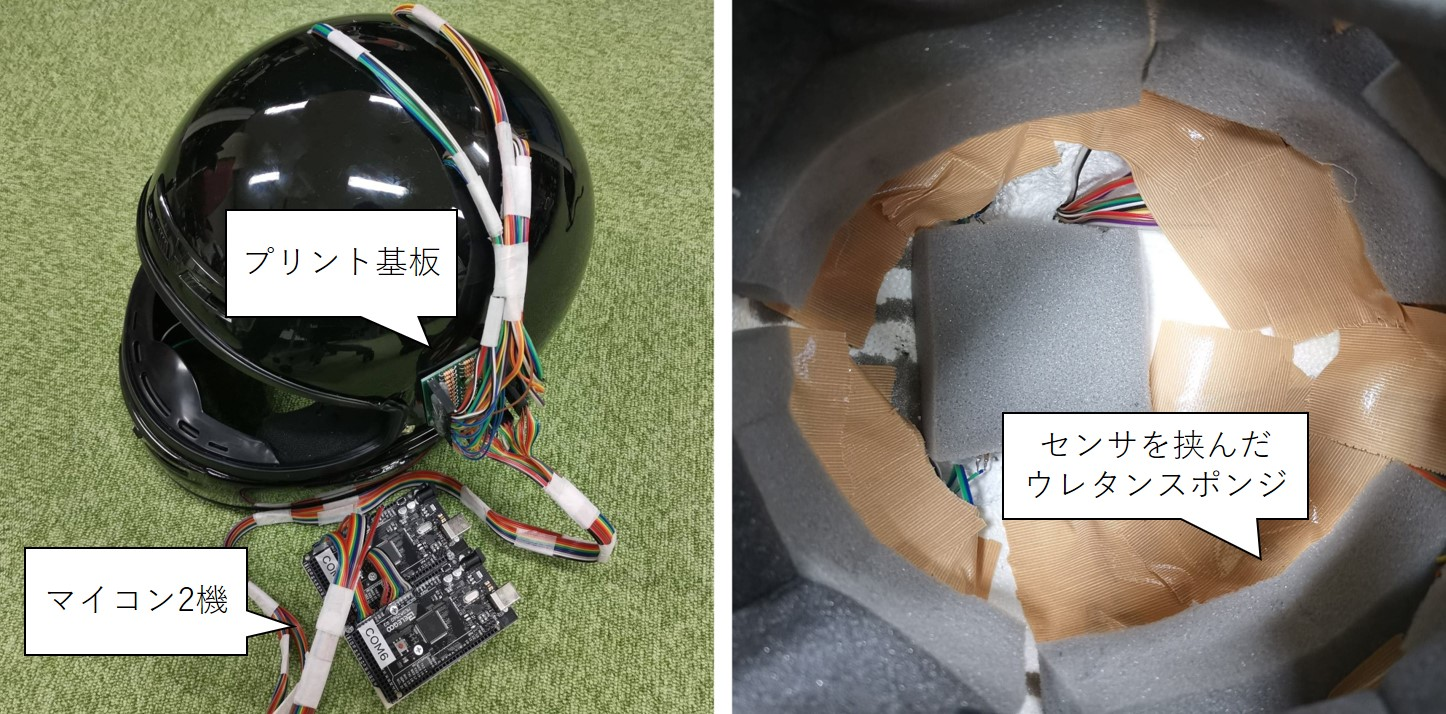
\includegraphics[width=1\linewidth]{met.eps}
%   \end{center}
%   \caption{実装したプロトタイプデバイス}
%   \label{device}
% \end{figure}

\bibliographystyle{junsrt}
\bibliography{references}

\end{document}
